\documentclass[11pt]{article}

% ── Packages ────────────────────────────────────────────────
\usepackage[margin=1in]{geometry}
\usepackage{amsmath, amssymb, amsthm}
\usepackage{booktabs}
\usepackage{graphicx}
\usepackage{hyperref}
\usepackage{natbib}
\usepackage{setspace}
\usepackage{microtype}
\usepackage{enumitem}
\usepackage{caption}
\usepackage{subcaption}
\usepackage{xcolor}
\usepackage{float}
% code packages
\usepackage{listings}
\usepackage{inconsolata}
\lstset{basicstyle=\ttfamily\footnotesize,breaklines=true}
\usepackage{csvsimple}
\usepackage{booktabs}

% ── Hyperref setup ──────────────────────────────────────────
\hypersetup{
    colorlinks = true,
    linkcolor  = black,
    citecolor  = black,
    urlcolor   = blue
}

% ── Theorem environments ────────────────────────────────────
\newtheorem{theorem}{Theorem}
\newtheorem{proposition}{Proposition}
\newtheorem{lemma}{Lemma}
\newtheorem{corollary}{Corollary}
\theoremstyle{definition}
\newtheorem{definition}{Definition}
\newtheorem{assumption}{Assumption}
\theoremstyle{remark}
\newtheorem{remark}{Remark}

% ── Spacing ─────────────────────────────────────────────────
\onehalfspacing

% ── Title block ─────────────────────────────────────────────
\title{Love of Variety: July 2nd Update}
\author{Tate Mason}
\date{\today}

% ============================================================
\begin{document}
\maketitle
\thispagestyle{empty}

\section{Overview}

This document presents data facts and consumer patterns from the Nielsen
HomeScan data I have been working on. I am currently working across all markets
and focusing on single person households in an attempt to make shopping trends
as clean as possible. Yogurt flavors are divided into three bins: plain, berry,
and other. While these are broad, they appear to be relatively balanced in terms
of how long people consume them and how often they switch. I also shrink down to
4-7 oz. cups of yogurt, again in an effort to get a clean baseline.

I find that, after a switch, 99\% of households switch back, on average, to
their original flavor. I also see households staying on switched-to flavors for
about 2-3 periods before switching again. The data also shows 40\% of
households take the outside option in any given period (not buying yogurt).
These facts are encouraging and suggest that, at least in yogurt cups, there is
some preference for variety in consumption.

Below, I will list summary statistics with brief discussion and then follow that
with some graphical evidence of switching behavior.

\section{Summary Statistics}

As stated above, all markets are present at this point, but households are
subset to single person households. Further, to reiterate, flavor bins are
plain, berry, and other.

\begin{table}[htbp]
    \centering
    \caption{Descriptive Statistics}
    \label{tab:desc_stats}
    \begin{tabular}{lc}
        \toprule
        Statistic & Value \\
        \midrule
        \# Households               & 15440 \\
        Mean \# Times Observed      & 15.76 \\
        Yogurt Purchases            & 1.85 \\
        Mean Income                 & \$16,277 \\
        Median Income               & \$16,000 \\
        \% White                    & 81\% \\
        \% Black                    & 13\% \\
        \% Hispanic                 & 4\% \\
        \% Asian                    & 2\% \\
        \% Taking Outside Option          & 0.41 \\
        Mean Repeat Purchase Rate (Brand)   & 75\% \\
        Mean Repeat Purchase Rate (Flavor)  & 42\% \\
        W/in HH Brand Concentration & 55\% \\
        W/in HH Flavor Concentration& 41\% \\
        Mean Consecutive Buys per HH (Other) & 4.2  \\
        Mean Consecutive Buys per HH (Berry) & 4.2 \\
        Mean Consecutive Buys per HH (Plain) & 8.5 \\
        Mean \% Return to Past Flavor After Switch & 0.99 \\
        \bottomrule
    \end{tabular}
\end{table}

\ref{tab:desc_stats} Shows that about 42\% of the time, on average, households are
buying the same flavor. Further, a singular flavor only makes up 41\% of
consumption. However, brand is more constant, implying that households may buy
the same flavor within brand rather than swapping along that dimension to the
same degree.

The most popular flavor is plain, and sees the most average consecutive buys.
This statistic warrants further investigation, as it is purchased 8 consecutive
shopping trips while both berry and other are 4.2 consecutive trips. There are
two possible explanations here. First, plain yogurt people are plain yogurt
people and exhibit more state dependence. Second, there is a coding issue with
flavor which I need to continue to look into. We do however, see that all
flavors are similar in terms of how long they are switched to for, which is
shown in \ref{fig:heatmap}.

We do see that 99\% of households return to their last flavor, behavior which is
in line with what I had hoped to see from the households. 

\section{Figures}

\begin{figure}[htbp]
  \centering
  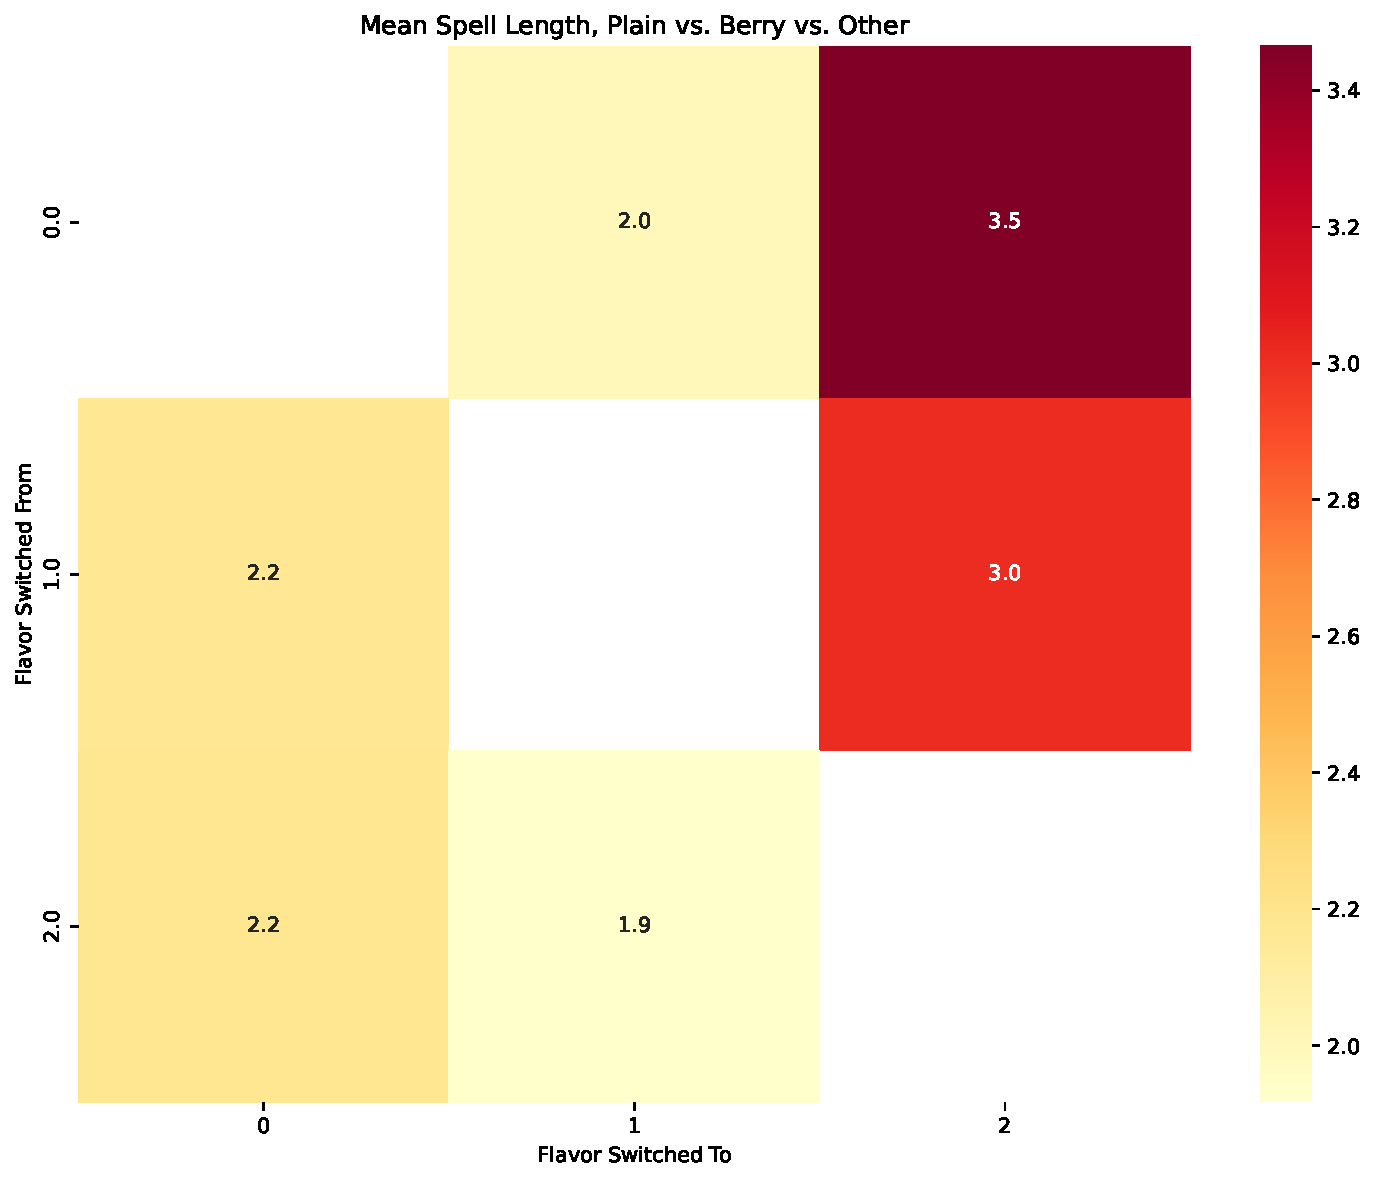
\includegraphics[width=\textwidth]{../../Output/Plots/3flav_heatmap.pdf}
  \label{fig:heatmap}
\end{figure}

As stated above, the three bins are close in terms of length of being switched
to. I also wanted to show the behavior when we make the flavor bins more
granular, giving each major flavor its own bin. Here, we see plain dominates,
highlighting the state dependence that plain yogurt people may have. This is
exhibited in \ref{fig:heatmap_granular} and \ref{fig:hist_granular}.

\begin{figure}[htbp]
  \centering
  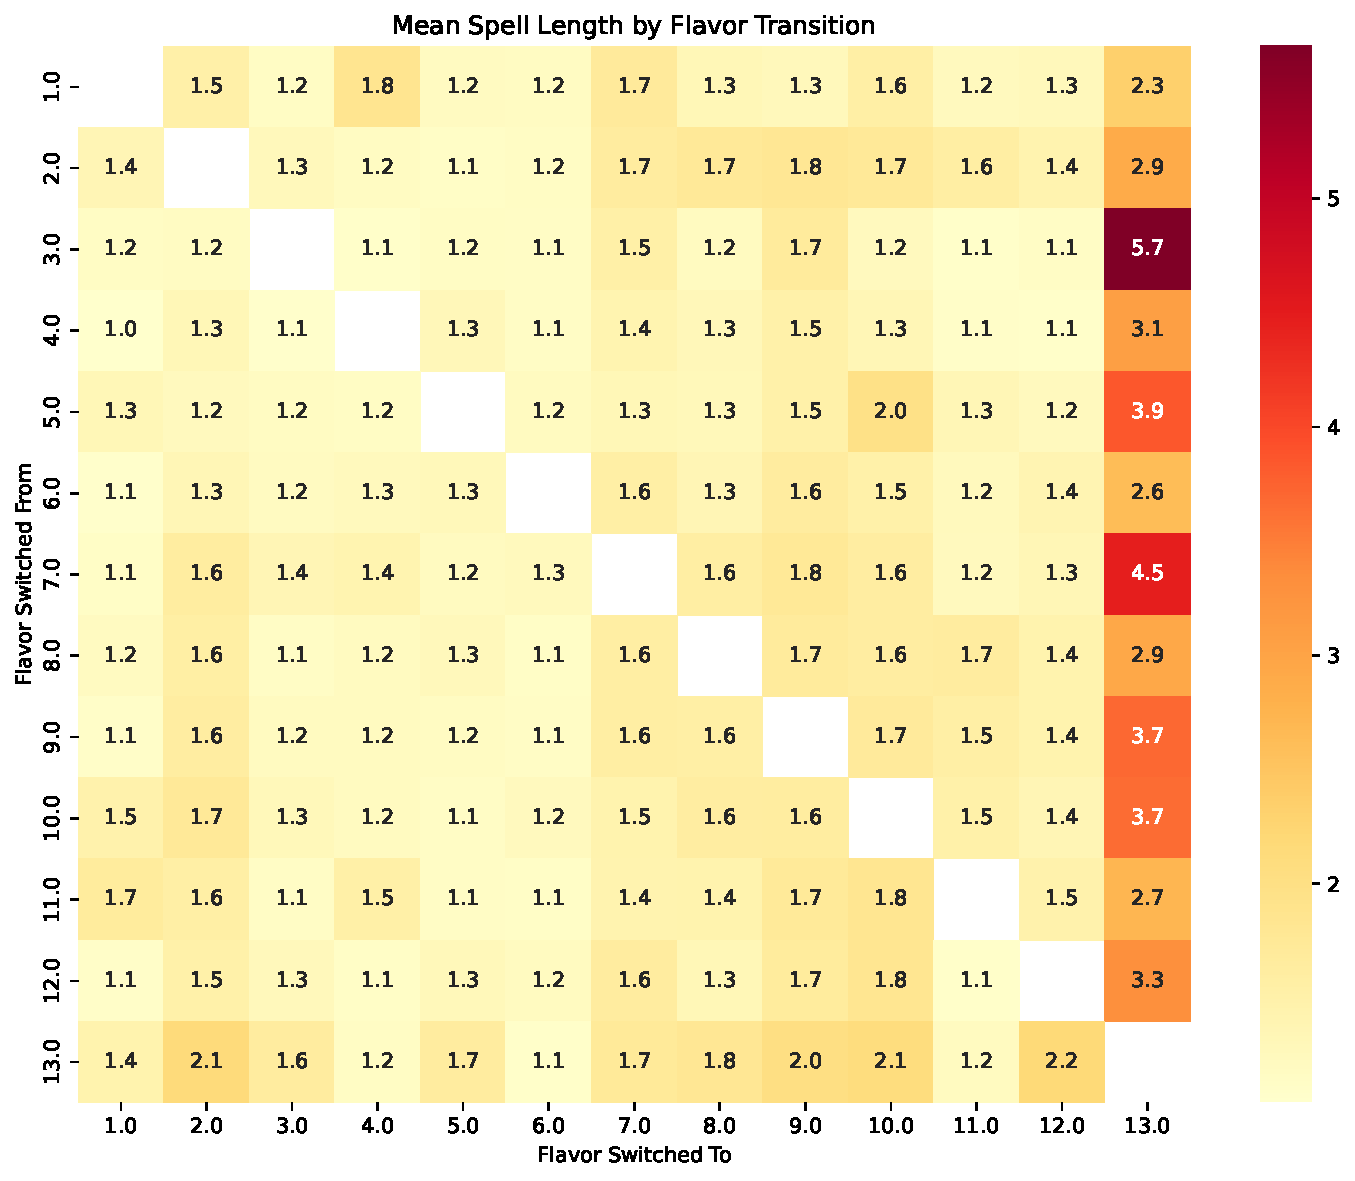
\includegraphics[width=\textwidth]{../../Output/Plots/run_length_heatmap.pdf}
  \label{fig:heatmap_granular}
\end{figure}

\begin{figure}[htbp]
  \centering
  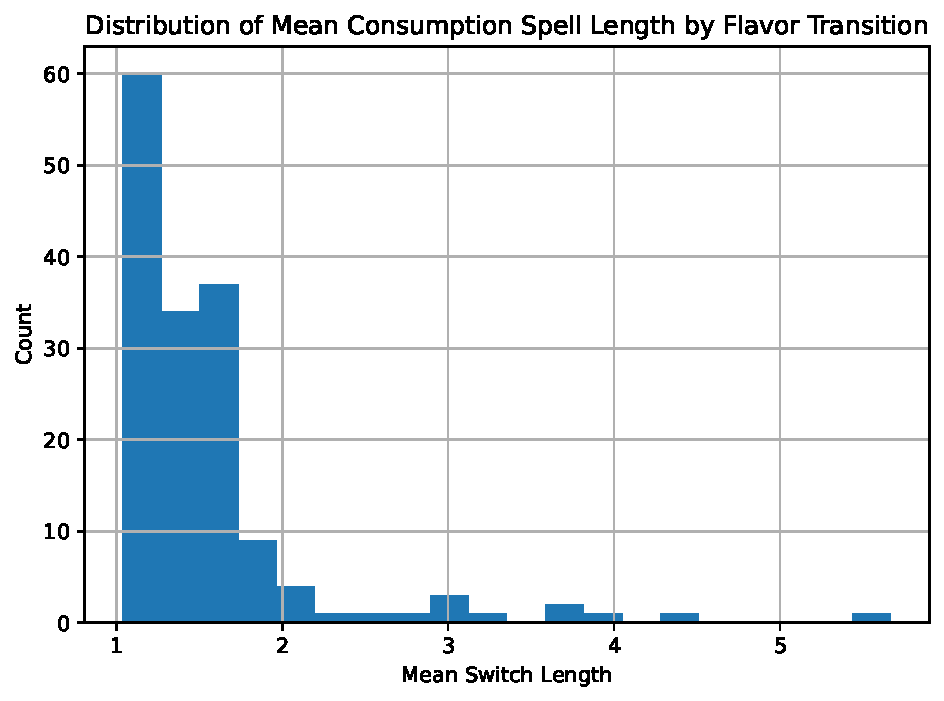
\includegraphics[width=\textwidth]{../../Output/Plots/run_length_hist.pdf}
  \label{fig:hist_granular}
\end{figure}

I am still playing with these bins, as I have to code them myself from flavor
codes given by Nielsen.

\section{Concluding and Next Steps}

From here, I plan to continue to find the right way to define the data and
recover more stats that could be used as micro-moments once I reach the
estimation stage. I also hope to move to other product categories like cereal
and ready to drink beverages. Any input is always appreciated.

\end{document}


